% -*- mode: latex; -*- mustache tags:  
\documentclass[10pt,twoside,english]{_support/latex/sbabook/sbabook}
\let\wholebook=\relax

\usepackage{import}
\subimport{_support/latex/}{common.tex}

%=================================================================
% Debug packages for page layout and overfull lines
% Remove the showtrims document option before printing
\ifshowtrims
  \usepackage{showframe}
  \usepackage[color=magenta,width=5mm]{_support/latex/overcolored}
\fi


% =================================================================
\title{Learning Object-Oriented Programming, Design and TDD with Pharo}
\author{Stéphane Ducasse}
\series{The Pharo TextBook Collection}

\hypersetup{
  pdftitle = {Learning Object-Oriented Programming, Design and TDD with Pharo},
  pdfauthor = {Stéphane Ducasse},
  pdfkeywords = {Introduction, programming, design, testing, Pharo, Smalltalk}
}


% =================================================================
\begin{document}

% Title page and colophon on verso
\maketitle
\pagestyle{titlingpage}
\thispagestyle{titlingpage} % \pagestyle does not work on the first one…

\cleartoverso
{\small

  Copyright 2017 by Stéphane Ducasse.

  The contents of this book are protected under the Creative Commons
  Attribution-ShareAlike 3.0 Unported license.

  You are \textbf{free}:
  \begin{itemize}
  \item to \textbf{Share}: to copy, distribute and transmit the work,
  \item to \textbf{Remix}: to adapt the work,
  \end{itemize}

  Under the following conditions:
  \begin{description}
  \item[Attribution.] You must attribute the work in the manner specified by the
    author or licensor (but not in any way that suggests that they endorse you
    or your use of the work).
  \item[Share Alike.] If you alter, transform, or build upon this work, you may
    distribute the resulting work only under the same, similar or a compatible
    license.
  \end{description}

  For any reuse or distribution, you must make clear to others the
  license terms of this work. The best way to do this is with a link to
  this web page: \\
  \url{http://creativecommons.org/licenses/by-sa/3.0/}

  Any of the above conditions can be waived if you get permission from
  the copyright holder. Nothing in this license impairs or restricts the
  author's moral rights.

  \begin{center}
    
\includegraphics[width=0.2\textwidth]{_support/latex/sbabook/CreativeCommons-BY-SA.pdf}
  \end{center}

  Your fair dealing and other rights are in no way affected by the
  above. This is a human-readable summary of the Legal Code (the full
  license): \\
  \url{http://creativecommons.org/licenses/by-sa/3.0/legalcode}

  \vfill

  % Publication info would go here (publisher, ISBN, cover design…)
  Layout and typography based on the \textcode{sbabook} \LaTeX{} class by Damien
  Pollet.
}


\frontmatter
\pagestyle{plain}

\tableofcontents*
\clearpage\listoffigures

\mainmatter

\chapter{Objects and classes}\label{cha:objectclass}
Pharo is a pure object-oriented programming language, i.e., everything in the system is an object i.e., an entity created by a class and reacting to messages.

This chapter presents key mechanisms that characterize object-oriented programming: \textit{objects}, \textit{classes},  \textit{messages} and \textit{methods}. We will also present \textit{distribution of responsibilities} which is one of the heart of object-oriented programming as well as \textit{delegation} and \textit{composition}. Each of these mechanisms will be used and illustrated again in this book.

We start explaining objects, classes, messages and methods with really simple examples. Then in the following chapter we will propose an example that illustrates what we can achieve by using objects of different classes. 

\textit{Objects} are created by \textit{classes} that are object factories: Classes define the structure and behavior of objects (in terms of methods) but each object has a specific state and identity that is unique and different from all other objects. A class defines \textit{methods} that specify how a \textit{message} is actually implemented. 
\section{Objects: Entities reacting to messages}
\textit{Instead of a bit-grinding processor ... plundering data structures, we have a universe of well-behaved objects that courteously ask each other to carry out their various desires.} {[}Ingall 81{]}

Object-oriented programming is about creating objects and interacting with objects by sending them \textit{messages}.

Objects are entities that communicate via messages and react to messages by executing certain tasks. Moreover objects hide the way they define these tasks: the client of an object send a message to an object and the system find the corresponding method to be executed. Messages specify what should be done and methods how it should be done. 
\subsection{Turtles as an example}
Imagine that we have a graphics turtle like a LOGO turtle. We do the following: create a turtle, send it messages to make it move, turn, and trace some drawings. Let us look at this in detail.
\subsection{Creating an object}
First we create a new turtle by sending the message \textcode{new} to the class \textcode{Turtle}. 

\begin{displaycode}{plain}
| t |
t := Turtle new. 
\end{displaycode}

A class is a cast for objects. All the objects, instances of a class, share the same characteristics and behavior. For example, all the turtle instances have a direction and understand messages to rotate and move. However, each turtle has its own value for its direction.
We say that all the instances of a class have the same instance variables but each as private value
for them. 
\subsection{Sending messages}
The only way to interact with objects is to send them \textit{messages}. 
In the following snippets we send messages

\begin{itemize}
\item to create an object , message \textcode{new},
\item to tell the turtle to turn, message \textcode{turn:}, and
\item to tell the turtle to move, message \textcode{go:}.
\end{itemize}

\begin{displaycode}{plain}
| t |
t := Turtle new. 
t turn: 90.
t go: 100.
t turn: 180. 
t go: 100.
\end{displaycode}

When an object receives a message, it reacts by performing some actions. An object can return a value, change its internal state, or send messages to other objects. Here the turtle will change its direction and it will interact with the display to leave a trail.
\subsection{Multiple instances: each with its own state. }
We can have multiple objects of the same class and each one has a specific state. Here we have two turles each one located to a specific position and pointing into its own direction. 

\begin{displaycode}{plain}
| t1 t2 |
t1 := Turtle new. 
t1 turn: 90.
t1 go: 100.
t1 turn: 180. 
t1 go: 100.
t2 := Turtle new.
t2 go: 100.
t2 turn: 40.
t2 go: 100.
\end{displaycode}
\section{Messages and Methods}
Messages specify \textit{what} the object should do and not how it should do it (this is the duties of methods). When we send the message \textcode{go:} we just specify what we expect the receiver to do.  Sending a message is similar to the abstraction provided by procedures or functions in procedural or functional programming language: it hides implementation details. However sending a message is much more than executing a sequence of instructions: it means that we have to find the method that should be executed in reaction to the message. 
\subsection{Message: what should be executed}
The message \textcode{square:} is send to a new turtle with 100 as argument. The message expresses what the receiver should do. 

\begin{displaycode}{plain}
Turtle new square: 100
\end{displaycode}
\subsection{Method: how we execute it}
The method definition \textcode{square:} below defines step by step what are the actions to be done in response to the message \textcode{square:}. It defines that to draw a square the turtle receiving the message \textcode{square:} (represented by \textcode{self}) should perform four times the following sequences of messages: move forward a distance (message \textcode{go:}), turn 90 degrees (using the message \textcode{turn:}).

\begin{displaycode}{plain}
square: size
	4 timesRepeat: [ self go: size; turn: 90 ]
\end{displaycode}

Note that finding the method corresponding to the message is done at runtime and depends on the object receiving the message.

\begin{coffee}
A message represents \textit{what} the object should do, while a method specifies \textit{how} the behavior is realized. 
\end{coffee}

An object can also send messages to other objects. For example, when a turtle draws a line, it sends messages to an object representing the line color and its length.


\begin{figure}

\begin{center}
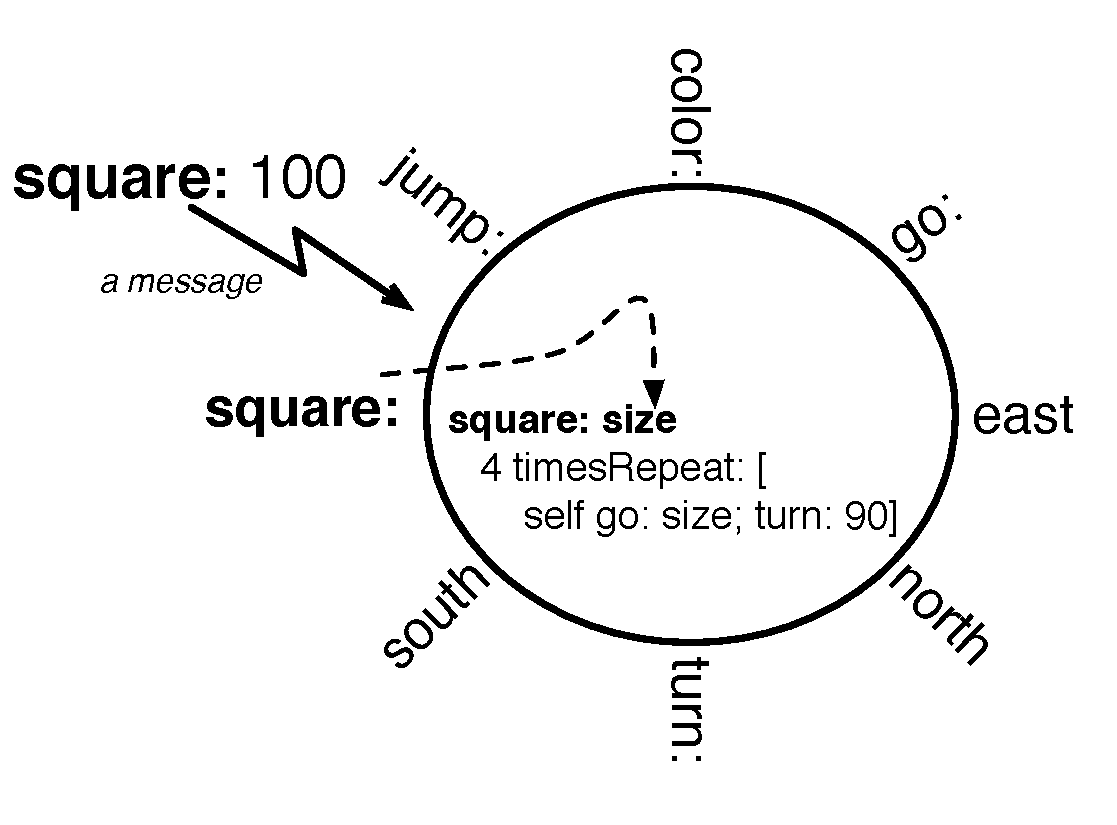
\includegraphics[width=0.5\textwidth]{/Users/ducasse/Workspace/FirstCircle/MyBooks/Bk-Writing/PharoBooks/LearningOOPWithPharoTrans/_result/pdf/Chapters/OOPNutshell/figures/basicMessageMethod.pdf}\caption{An object presents to the other objects an interface composed of a set of messages defining \textit{what} he can do. This behavior is realized by methods that specify \textit{how} the behavior is implemented. When a message is sent to an object a method with the message name (called selector) is looked up and executed. \label{basicMessageMethod}}\end{center}
\end{figure}


\begin{coffee}
An object is an entity that once created receives messages and performs some actions in reaction. When a message is sent to an object, a method with the message name is looked up and executed.
\end{coffee}
\section{An object is a protective entity}
An object is responsible of the way it realizes its reaction to a message.  It \textit{offers services} but \textit{hides} the way they are implemented (see Figure \ref{fig:encapsulationAtWork2}). We do not have to know how the method associated with the message selector is implemented.  Only the object knows the exact definition of the method.  This is when we define the method \textcode{square:} that defines how a turtle draws a square of a given size, that we focus on \textit{how} a turtle draws a square. Figure \ref{fig:encapsulationAtWork2} shows the message and the method \textcode{square:}. The method \textcode{square:} defines how to draw step by step a square, however the object only offers the message square: and does not show it implementation.

\begin{important}
An object presents to the other objects an \textit{interface} (i.e., a set of messages) defining \textit{what} the object can do. This behavior is realized by methods that specify \textit{how} the behavior is implemented. To perform something useful some data are most of the time required. Data are only accessed by the methods.
\end{important}

From a turtle \textit{user} point of view, the only relevant information is that the turtle effectively receiving the message \textcode{square:} executes the method that draws a square. So changing the definition of the \textcode{square:} method  to the one below does not have any consequence on the methods that call it. Figure \ref{fig:encapsulationAtWork2} illustrates this point.

\begin{displaycode}{plain}
square: s
   "Make the receiver draw a square of size s"

   self go: s; turn: 90; go: s; turn: 90.
   self go: s; turn: 90; go: s; turn: 90
\end{displaycode}


\begin{figure}

\begin{center}
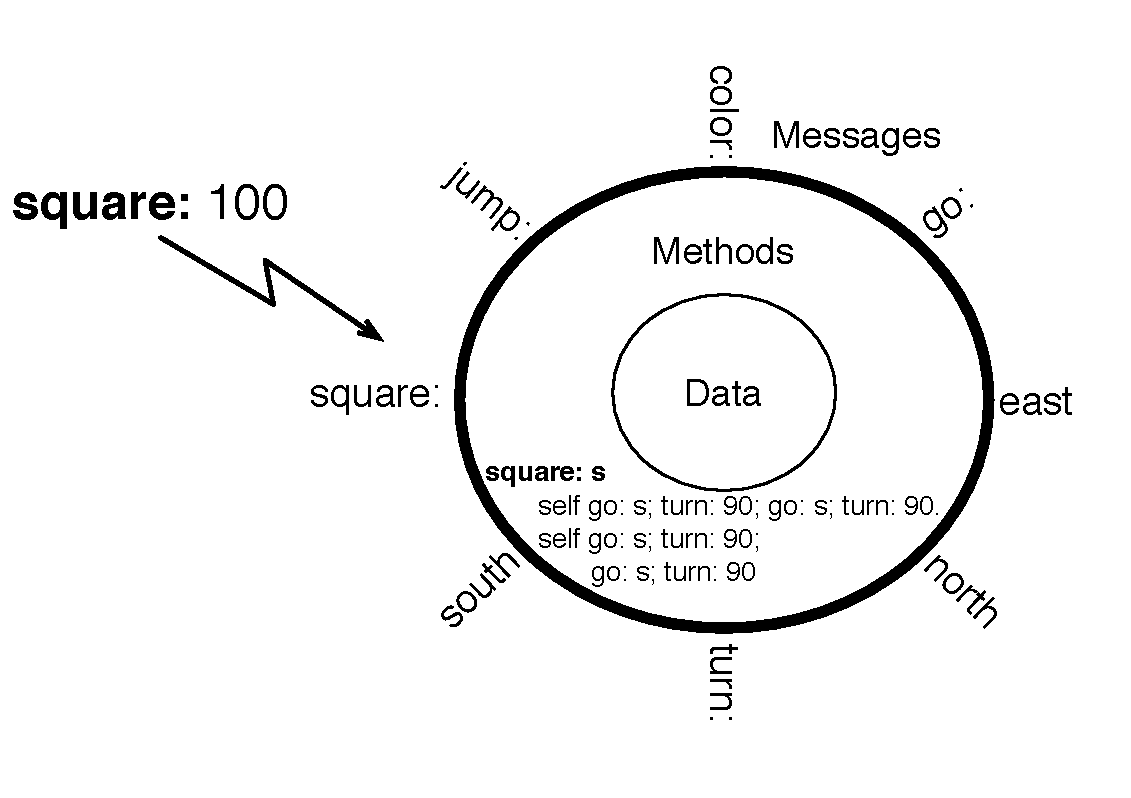
\includegraphics[width=0.5\textwidth]{/Users/ducasse/Workspace/FirstCircle/MyBooks/Bk-Writing/PharoBooks/LearningOOPWithPharoTrans/_result/pdf/Chapters/OOPNutshell/figures/encapsulationAtWork2.pdf}\caption{The message \textcode{square:} can be implemented differently. This different implementation does not impact the sender of the message who is not concerned by the internals of the object.\label{fig:encapsulationAtWork2}}\end{center}
\end{figure}


Hiding the internal representation is not limited to object-oriented programming but it is central to object-oriented programming. 

\begin{important}
An object is responsible of the way it realizes its reaction to a message. It offers services and hides the way they are implemented.
\end{important}
\section{An object protects its data}
An object holds some \textit{private data} that represents its state (see Figure \ref{fig:objectOne}). Moreover, it controls its state and should not let other objects play directly with them because this could let him into an inconsistent state.  For example, you do not want to somebody else plays with the data of your bank account directly and really want to control your transaction.

For example, a LOGO turtle can be represented by a position, a direction and a way to indicate if its pen is up or down. But, we cannot directly access these data and change them. For that we have to use the set of messages proposed by a turtle. These methods constitute the \textit{interface} of an object. We say that the object state is \textit{encapsulated}, this means that not everybody can access it. In fact, object-oriented programming is based on encapsulation, i.e., the fact that per default objects are the only ones that can access their own state.


\begin{figure}

\begin{center}
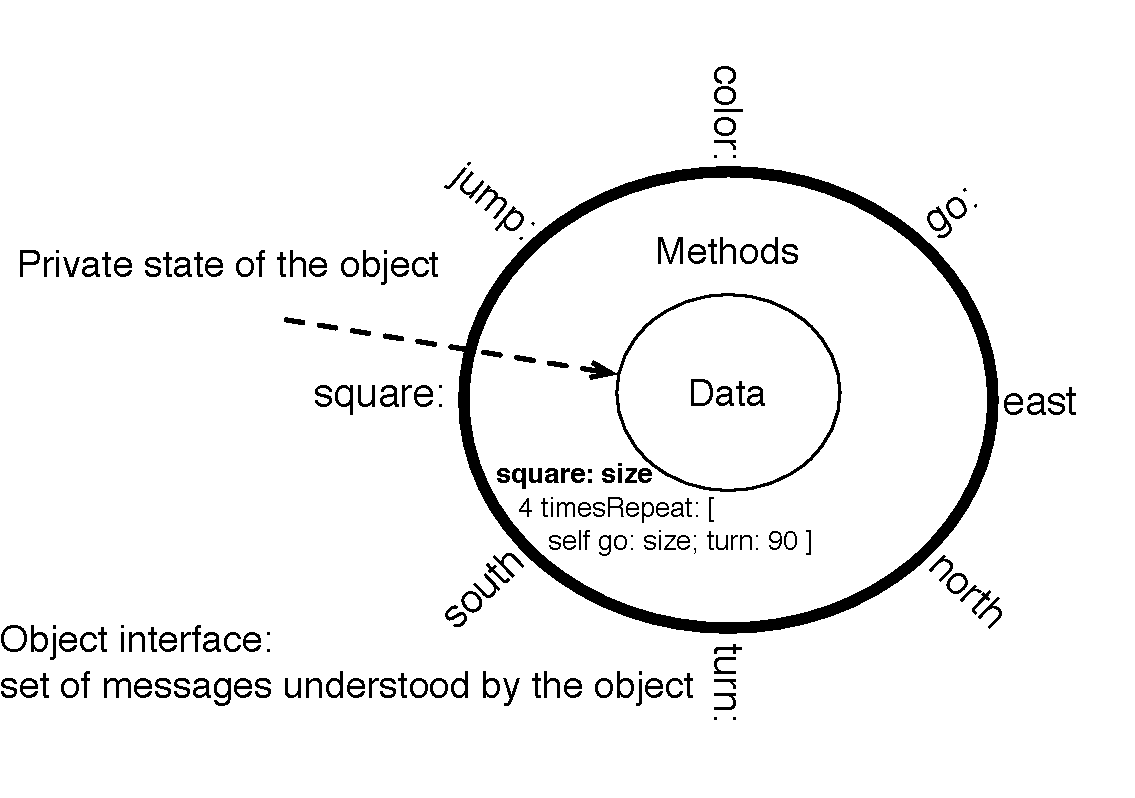
\includegraphics[width=0.45\textwidth]{/Users/ducasse/Workspace/FirstCircle/MyBooks/Bk-Writing/PharoBooks/LearningOOPWithPharoTrans/_result/pdf/Chapters/OOPNutshell/figures/privateData.pdf}\caption{A turtle is an object which has an interface, i.e., a set of messages to which it can reply and a private state that only its methods can access.\label{fig:objectOne}}\end{center}
\end{figure}


In Pharo, a client cannot access the state of an object if the object does not define a method to access it.  Moreover, clients should not  rely on the internal representation of an object because an object is free to change the way it  implements its behavior. Exposing the internal state of an object by defining methods providing access to the object data weakens the control that an object has over its own state.


\begin{figure}

\begin{center}
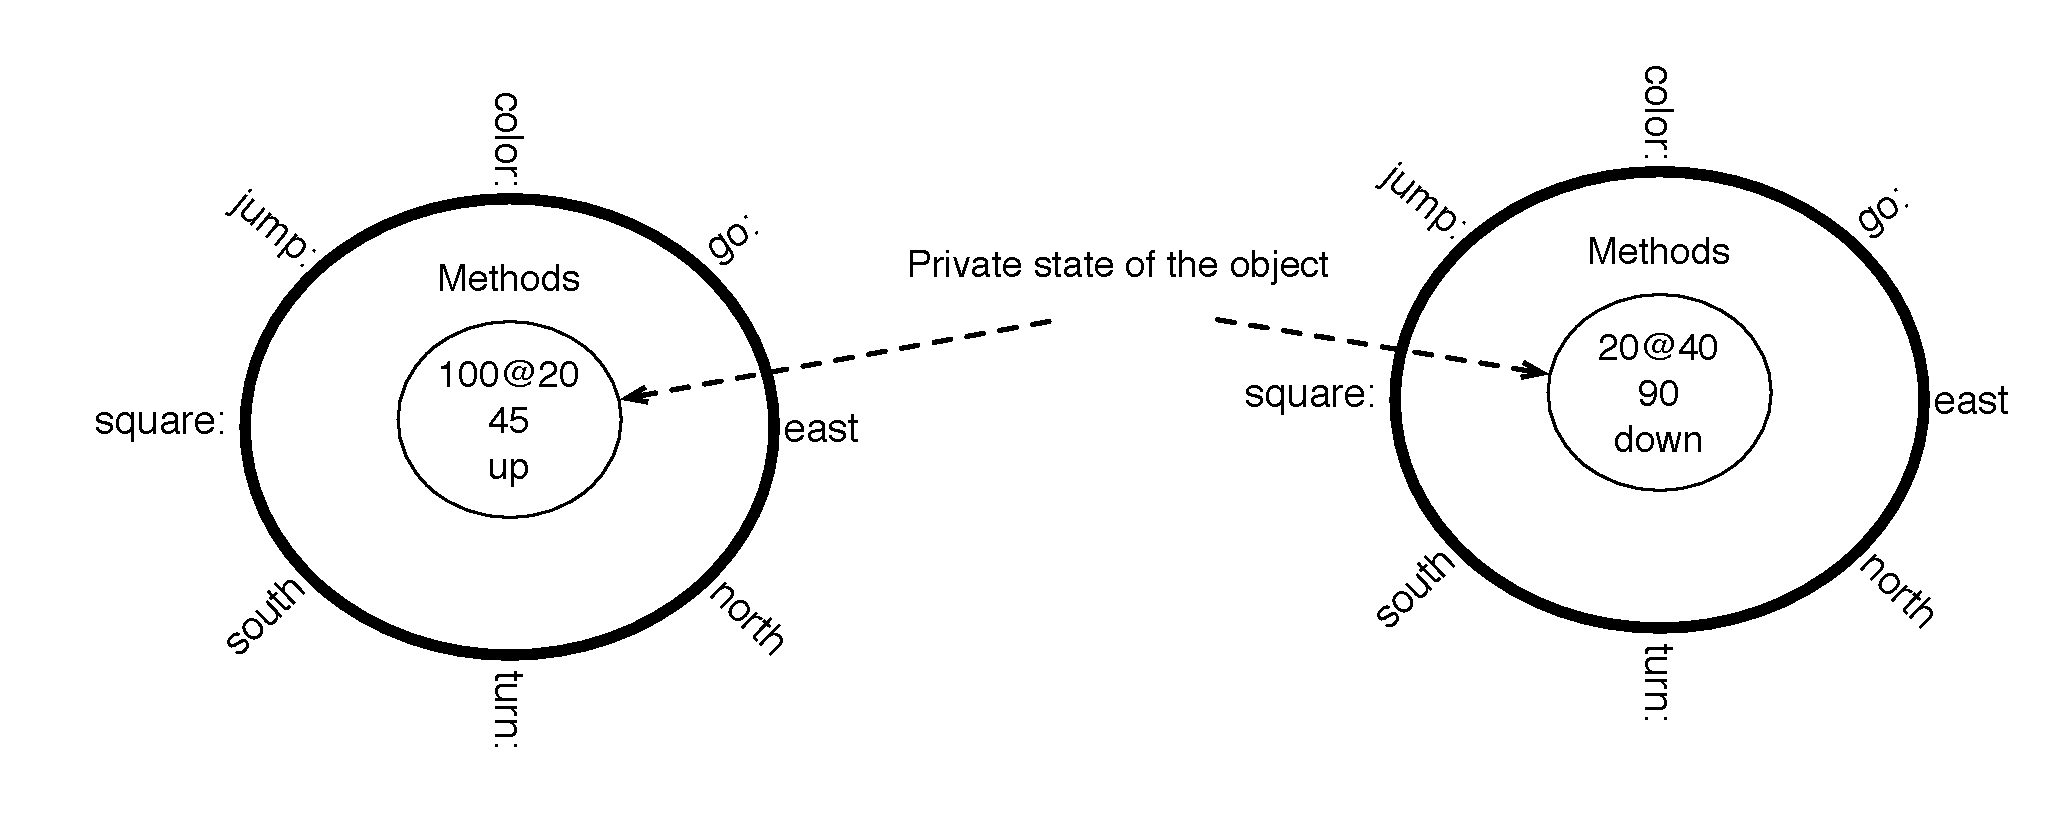
\includegraphics[width=0.7\textwidth]{/Users/ducasse/Workspace/FirstCircle/MyBooks/Bk-Writing/PharoBooks/LearningOOPWithPharoTrans/_result/pdf/Chapters/OOPNutshell/figures/privateDataTwoInstances.pdf}\caption{Two turtles have the same interface, i.e., set of messages  being understood but they have \textit{different} private state representing their  direction, position and pen status.\label{fig:twoInstances}}\end{center}
\end{figure}


\begin{important}
An object holds some \textit{private} data that represents its \textit{internal} state. Each object has its own state. Two objects of the same class share the same \textit{interface} but have their own private state.
\end{important}
\section{With counters}
Now that you got the main point of objects, we can see that it applies to everything. In Pharo \textit{everything} is an object. In fact there is \textit{nothing} else, only objects. Here is a little program with counters. 

We create two counters that we store in variables \textcode{c1} and \textcode{c2} instances of the class \textcode{Counter}. Each counter has its own state but exhibits the same behavior as all the counters defined by the class \textcode{Counter}: 

\begin{itemize}
\item when responding to the message \textcode{count}, it returns its value,
\item when responding to the message \textcode{increment}, it increment one to its current value. 
\end{itemize}

\begin{displaycode}{plain}
| c1 c2 |
c1 := Counter new.
c2 := Counter new.
c1 count.
>>> 0
c1 increment.
c1 increment.
c1 count. 
>>> 2
c2 count.
>>> 0
c 2 increment.
c2 count. 
>>> 1
\end{displaycode}
\section{A class: blueprint or factory of objects}
A class is a mold or cast of objects. A class specifies two important aspects of their instances:

\begin{itemize}
\item Instance \textbf{structure}. All the instances of a class will have the same structure expressed in terms of \textit{instance variables}. Pay attention that the variables are the same for all the instances of a class but not their values. Each instance has specific values for its instance variables.
\item Instance \textbf{behavior}. All the instances share the same behavior even if this one can be different because applied on different values. 
\end{itemize}

\begin{important}
A class is as a blueprint for its instances. It is a factory of objects. All objects will have the same structure and share a common behavior. 
\end{important}

Let us illustrate this with the class \textcode{Counter}.
\subsection{Object structure}
Let us study the \textcode{Counter} class definition.  

\begin{displaycode}{plain}
Object subclass: #Counter
	instanceVariableNames: 'count'
	classVariableNames: ''
	package: 'LOOP'
\end{displaycode}

The expresion \textcode{Object subclass: \#Counter} indicates that the class \textcode{Counter} is a subclass of the class \textcode{Object}.
It means that counter instances understand the messages defined also by the class \textcode{Object}. In Pharo, classes should at least be a subclass of the class \textcode{Object}. You will learn more about subclassing and inheritance in Chapter \ref{cha:inheritance}.

Then the class \textcode{Counter} defines that all the instances will have one instance variable named \textcode{count} using the expression \textcode{instanceVariableNames: 'count'}. And each instance of the class \textcode{Counter} will have a \textcode{count} variable with a \textit{different} value as we showed in the examples above.

Finally the class is defined in the package \textcode{'LOOP'}. A package is a kind of folder containing multiple classes. 
\subsection{Object behavior}
In addition a class is the place that groups the behavior of its instances. Indeed since all the instances of the class share the \textit{same} behavior definitions, such behavior is defined and grouped in a class.

For counters, the class defines how to retrieve the counter value, how to increment 
and decrement the count as used in the messages in the previous code snippets.

Here is the definition of the \textbf{method} \textcode{increment}. 
It simply adds one to the instance variable \textcode{count}.

\begin{displaycode}{plain}
Counter >> increment
	count := count + 1
\end{displaycode}

When we send a message to a counter for example in the expression \textcode{c1 increment}, 
the method \textcode{increment} will be applied on \textit{that} specific object \textcode{c1}.
In the expression \textcode{c1 increment}, \textcode{c1} is called the \textbf{receiver} of the message \textcode{increment}. 

In the method \textcode{increment},  the variable \textcode{count} refers to the variable of the \textbf{receiver} of the message. 

\begin{coffee}
A class defines methods that specify the behavior of all the instances created by the class.
\end{coffee}

Multiple methods can accessed to the instance variables of the receiver. For example the methods \textcode{increment}, \textcode{count:} \textcode{decrement} and \textcode{printOn:} all access the instance variable \textcode{count} of the receiver to perform different computation. 

\begin{displaycode}{plain}
Counter >> count: anInteger
	count := anInteger
\end{displaycode}

\begin{displaycode}{plain}
Counter >> decrement
	count := count - 1
\end{displaycode}

\begin{displaycode}{plain}
Counter >> printOn: aStream
   super printOn: aStream.
   aStream nextPutAll: ' with value: ', self count printString.
\end{displaycode}

For example, once the following program is executed the count  instance variable of the counter \textcode{c2} will hold the value 11, since the method \textcode{count:} will set its value to 10, and \textcode{increment} will set it to 11 and 12 and finally \textcode{decrement} will set it to 11. 

\begin{displaycode}{plain}
| c2 |
c2 := Counter new.
c2 count: 10.
c2 increment.
c2 increment.
c2 decrement.
\end{displaycode}
\subsection{Self is the message receiver}
Imagine that now we would like to send a message to the object that receives the message itself. We need a way to refer to this object. Pharo defines a special variable for this exact purpose: \textcode{self}. 

\begin{important}
\textcode{self} always refers to the message receiver that is currently executed.
\end{important}

For example we can implement the method \textcode{incrementByTwo} as follows:

\begin{displaycode}{plain}
Counter >> incrementByTwo
	self increment. 
	self increment
\end{displaycode}

When we execute the expression \textcode{c1 incrementByTwo}, during the execution of the method \textcode{incrementByTwo}, \textcode{self} refers to \textcode{c1}. 

We will explain  how a method is found when a message is sent but first we should explain inheritance, i.e., how a class is defined incrementally from a root class and all this will be explained  in Chapter \ref{cha:inheritance}.
\section{Class and instances are really different}
Classes and objects are different objects; they understand different messages. 

For example, sending \textcode{new} to the \textcode{Counter} class returns a newly created counter, while sending \textcode{new} to a counter results in an error. In the opposite way, sending \textcode{increment} to the class \textcode{Counter} leads also to an error because the class \textcode{Counter} is a factory of objects not the objects themselves. 

A class is a factory of objects. A class creates instances. An instance does not create other instances of the class.

\begin{coffee}
A class describes the structure (instance variables) and the behavior (methods) of \textit{all} its instances. The state of an instance is the value of its instance variables and it is specific to one single object while the behavior is shared by all the instances of a class.
\end{coffee}
\section{Conclusion}
In this chapter you saw that: 

\begin{itemize}
\item An object is a computer entity that once created receives messages and performs some actions in reaction.
\item An object has an unique identity.
\item An object holds some private data that represent its internal state.
\end{itemize}

\begin{itemize}
\item A class is a factory of objects: It \textit{describes} the internal structure of all its instances by means of instance variable. 
\item All objects of the same class share the same behavior, i.e., the same method definitions.
\item Instance variables are accessible by all the methods of a class. Instance variables have the same lifetime than the object to which they belong to.
\item In Pharo , instance variables cannot be accessed from outside of an object. Instance variables are only accessible from the methods of the class that define them.
\item Methods define the behavior of all the instances  of the class they belong to.
\end{itemize}
\chapter{Revisiting objects and classes}
In the previous chapter we presented objects and classes via simple examples. In this chapter we introduce a little bit more elaborated example: a little file system where we revisit everything and extend it to explain \textit{late binding}, \textit{distribution of responsibilities} and \textit{delegation}. The file example will be extended to present \textit{inheritance} in Chapter \ref{cha:inheritance}.
\section{A simple and naive file system}
We start to present a simple example that we use to present and explain the concepts: a simple and naive file system as shown in Figure \ref{figdirectories}. 
What the diagram shows is that we have:

\begin{itemize}
\item files that also have a name and a contents. Here we get three different files \textcode{Babar}, \textcode{Astroboy} and \textcode{tintinEtLesPicaros}.
\item directories that have a name and can contain other files or directories. Here we get the \textcode{manga}, \textcode{comics}, \textcode{oldcomics} and \textcode{belgiumSchool} directories. Directories can be nested: \textcode{comics} contains three repositories. The \textcode{belgiumSchool} directory contains \textcode{tintinEtLesPicaros}. 
\end{itemize}


\begin{figure}

\begin{center}
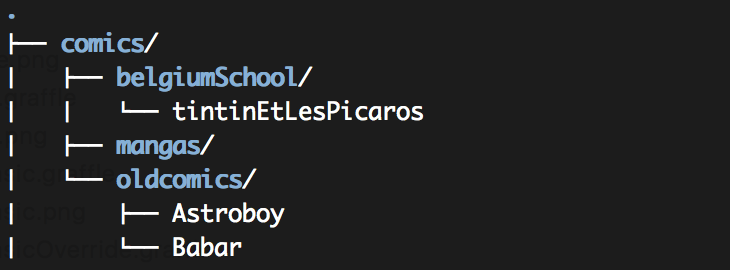
\includegraphics[width=0.5\textwidth]{/Users/ducasse/Workspace/FirstCircle/MyBooks/Bk-Writing/PharoBooks/LearningOOPWithPharoTrans/_result/pdf/Chapters/OOPNutshell/figures/comicsFileTree.png}\caption{Some directories and files organised in a file system.\label{figdirectories}}\end{center}
\end{figure}

\section{Studying a first scenario}
Since what we want to develop may be a bit unclear for us, let us define first an example. In the rest of this book we will code such examples as tests that can automatically be executed. For now it would make the discourse too complex, so we just use little code examples. 

We create two directories.

\begin{displaycode}{plain}
| dComics dOldComics dManga |
dComics := MFDirectory new name: 'comics'.
dOldComics := MFDirectory new name: 'oldcomics'.
\end{displaycode}

We add the oldcomics folder to comics and we check that the parent children relationship is well set. 

\begin{displaycode}{plain}
	...
dComics addElement: dOldComics. 
dOldComics parent == dComics
>>> true
\end{displaycode}

Here we verify that the parent of \textcode{dOldComics} is \textcode{dComics}: the message \textcode{ == } checks that the receiver is the same object than the argument.  

You can also inspect the receiver as follows and if you click on the instance variable parent of the receiver you should obtain the situation depicted by Figure \ref{inspectingComics}.

\begin{displaycode}{plain}
	...
dOldComics inspect
\end{displaycode}


\begin{figure}

\begin{center}
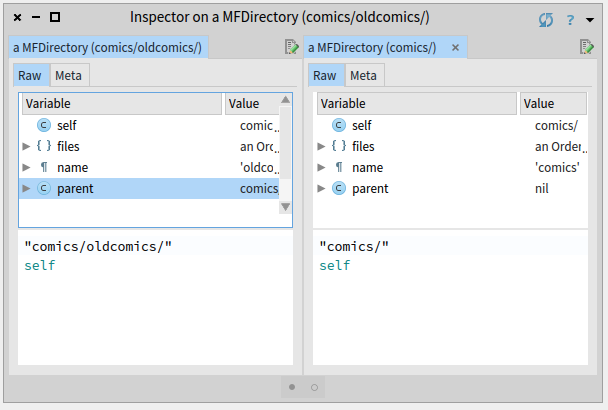
\includegraphics[width=0.7\textwidth]{/Users/ducasse/Workspace/FirstCircle/MyBooks/Bk-Writing/PharoBooks/LearningOOPWithPharoTrans/_result/pdf/Chapters/OOPNutshell/figures/inspectingComics.png}\caption{Inspecting \textcode{dOldComics} and clicking on the \textcode{parent} variable. \label{inspectingComics}}\end{center}
\end{figure}


We continue with some queries.

\begin{displaycode}{plain}
	...
dComics parent
>>> nil
\end{displaycode}

Here we verify that \textcode{dOldComics} is comprised in the children of \textcode{dComics}. 

\begin{displaycode}{plain}
	...
dComics children includes: dOldComics. 
>>> true
\end{displaycode}

We create a new repository and we check that once added to a parent repository, it is included in the 
children.

\begin{displaycode}{plain}
dManga := MFDirectory new name: 'manga'.
dComics addElement: dManga. 
dComics children includes: dManga
>>> true
\end{displaycode}


\begin{figure}

\begin{center}
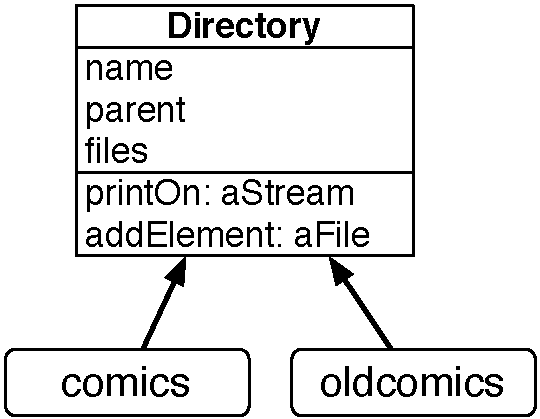
\includegraphics[width=0.35\textwidth]{/Users/ducasse/Workspace/FirstCircle/MyBooks/Bk-Writing/PharoBooks/LearningOOPWithPharoTrans/_result/pdf/Chapters/OOPNutshell/figures/DirectoryAndInstancesV0.pdf}\caption{The \textcode{Directory} class and some instances (directories).\label{directories}}\end{center}
\end{figure}

\section{Defining a class}
Let us start by defining the directory class. 

\begin{displaycode}{plain}
Object subclass: #MFDirectory
	instanceVariableNames: 'parent name files'
	classVariableNames: ''
	package: 'MyFS'
\end{displaycode}

When we create a directory, its files is an empty ordered collection. This is what we express in the following method \textcode{initialize}.

\begin{displaycode}{plain}
MFDirectory >> initialize
	files := OrderedCollection new
\end{displaycode}

A newly created object is sent the message \textcode{initialize} just after its creation. Therefore the \textcode{initialize} method is executed. 

Now we can write the method \textcode{addElement:}. 
(To keep things simple, note that we consider that when a file is added to a directory, it was not belonging to a another directory. This behavior could be implemented by \textcode{aFile moveTo: aDirectory})
Adding a file to a directory means: (1) that the parent of the file is changed to be the directory to which it is added, (2) that the added file is added to the list of files contained in the directory.

\begin{displaycode}{plain}
MFDirectory >> addElement: aFile
	aFile parent: self. 
	files add: aFile
\end{displaycode}

Note that the method name \textcode{addElement:} is not nice but we chose it on purpose so that you do not believe that delegating
requires that the methods have the same name. An object can delegate its part of duties to another object by simply passing a message. 

We should then define the methods \textcode{name:}, \textcode{parent:}, \textcode{parent}, and \textcode{children} to be able to run our example.

\begin{displaycode}{plain}
MFDirectory >> name: aString
	name := aString
\end{displaycode}

\begin{displaycode}{plain}
MFDirectory >> parent: aFile
	parent := aFile
\end{displaycode}

\begin{displaycode}{plain}
MFDirectory >> parent
	^ parent
\end{displaycode}

\begin{displaycode}{plain}
MFDirectory >> children
	^ files
\end{displaycode}

With such method definitions, our little example should run. It should not print the same results because we did not change the printing of the objects yet. 
\subsection{A first little analysis}
When we look at the implementation of the method to add a file to a directory we see that the class \textcode{MFDirectory} used another class \textcode{OrderedCollection} to store the information about the files it contains. An ordered collection is a quite complex object: it can insert, remove elements, grow its size, and many more operations. 

We say that the class \textcode{MFDirectory} delegates a part of its duties (to keep the information of the files it contains) to the class \textcode{OrderedCollection}. In addition, when an object is executed, the object to which it may delegate part of its computation may change dynamically. 

Such behavior is not specific to object-oriented programming, in procedural languages we can call another function defined on a data structure. 
Now with object-oriented programming, there is a really important point: an object will send messages to other objects (even from the same class) and such message send will use the message offered by the receiver. There is normally no way for an object to access the internal structure of another object.
\section{Printing a directory}
Now we would like to get the directory printed in a better way. Without too much explanation, you should know that the method \textcode{printOn: astream} of an object is executed when the system or we send the message \textcode{printString} to an object. So we can specialise it. 

The argument passed to the method \textcode{printOn:} is a stream. A stream is an object in which we can store information one after the other in sequence using the message \textcode{\textless{}\textless{}}. The argument of \textcode{\textless{}\textless{}} should be a sequence of objects such as string (which is a sequence of characters).

\begin{displaycode}{plain}
MFDirectory >> printOn: aStream
	aStream << name
\end{displaycode}

Let us try. 

\begin{displaycode}{plain}
| el1 el2 |
el1 := MFDirectory new name: 'comics'.
el2 := MFDirectory new name: 'oldcomics'.
el1 addElement: el2.
el1 printString
>>> 'comics'
\end{displaycode}

\begin{displaycode}{plain}
	...
el2 printString
>>> 'oldcomics'
\end{displaycode}

What would be nice is to get the full path so that we can immediately understand the configuration.
For example we would like to  finish with a '/' to indicate that this is a directory as with the ls command on unix. 

\begin{displaycode}{plain}
| el1 el2 |
el1 := MFDirectory new name: 'comics'.
el2 := MFDirectory new name: 'oldcomics'.
el1 addElement: el2.
el1 >> printString.
>>>'comics'
\end{displaycode}

\begin{displaycode}{plain}
	...
el2 printString
>>> 'comics/oldcomics/'
\end{displaycode}

A possible definition is the following one:

\begin{displaycode}{plain}
MFDirectory >> printOn: aStream
	parent isNil 
		ifFalse: [ parent printOn: aStream ].
	aStream << name.
	aStream << '/'
\end{displaycode}


\begin{figure}

\begin{center}
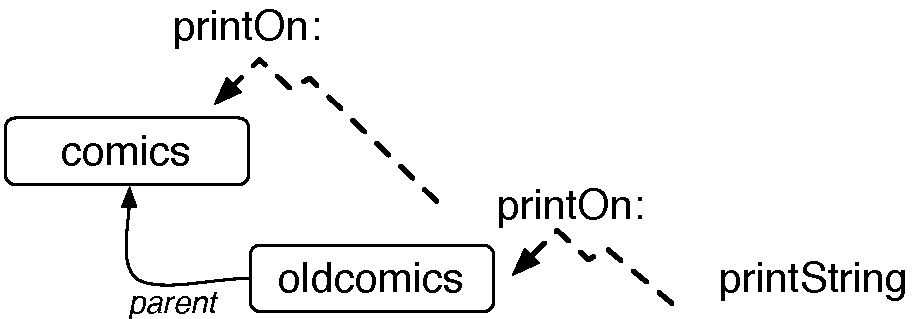
\includegraphics[width=0.55\textwidth]{/Users/ducasse/Workspace/FirstCircle/MyBooks/Bk-Writing/PharoBooks/LearningOOPWithPharoTrans/_result/pdf/Chapters/OOPNutshell/figures/InstancesRecursion.pdf}\caption{Navigating an object graph by sending message to different objects. \label{InstancesRecursion}}\end{center}
\end{figure}


Try it and it should print the expected results.
What do we see with this definition: it is a kind of recursive definition. The name of a directory is in fact the concatenation (here we just add in the stream but this is the same. ) of the name of its parents (as shown in Figure \ref{InstancesRecursion}).
Similar to a recursive function navigating a structure composed of similar elements (like a linked-list or any structure defined by induction), each parent receives and executes another time the \textcode{printOn:} method and returns the name for its part.
\section{Adding files}
Now we want to add files. Once we will have defined files we will be able to have a graph of objects of different kinds represent our file system with directories and files as shown in Figure \ref{Instances}.


\begin{figure}

\begin{center}
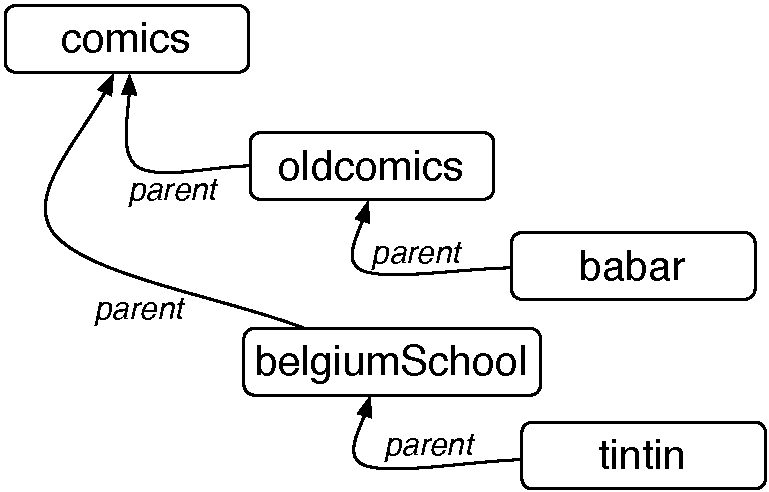
\includegraphics[width=0.45\textwidth]{/Users/ducasse/Workspace/FirstCircle/MyBooks/Bk-Writing/PharoBooks/LearningOOPWithPharoTrans/_result/pdf/Chapters/OOPNutshell/figures/Instances.pdf}\caption{A graph of objects to represent our file system. \label{Instances}}\end{center}
\end{figure}

\subsection{An example first}
Again let us start with an example.  A file should contain some contents. 

\begin{displaycode}{plain}
| el1 dOldComics |
el1 := MFFile new name: 'astroboy'; contents: 'The story of a boy turned into a robot that saved the world'.
dOldComics := MFDirectory new name: 'oldcomics'.
dOldComics addElement: el1. 
el1 printString.
>>>
'oldcomics/astroboy'
\end{displaycode}


\begin{figure}

\begin{center}
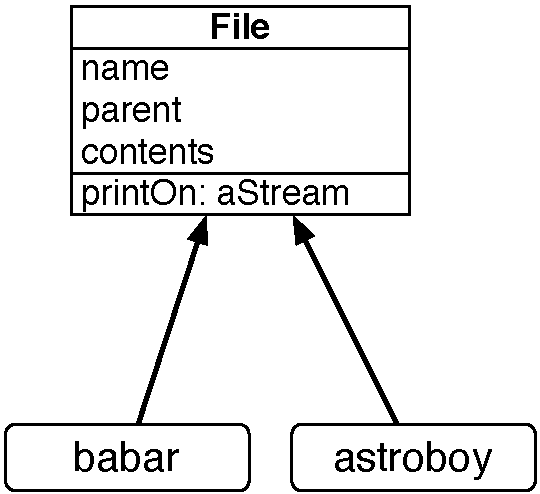
\includegraphics[width=0.35\textwidth]{/Users/ducasse/Workspace/FirstCircle/MyBooks/Bk-Writing/PharoBooks/LearningOOPWithPharoTrans/_result/pdf/Chapters/OOPNutshell/figures/FileV0.pdf}\caption{A new class and its instances.\label{FileV0}}\end{center}
\end{figure}

\subsection{A new class definition}
Again a file needs a name, a parent and in addition a contents.

We define the class \textcode{MFFile} as follows and illustrated in Figure \ref{FileV0}.
Note that this solution is not satisfactory and we will propose a much better one later.

\begin{displaycode}{plain}
Object subclass: #MFFile
	instanceVariableNames: 'parent name contents'
	classVariableNames: ''
	package: 'MyFS'
\end{displaycode}

As for the directories we initialize the contents of a file with a default value. 

\begin{displaycode}{plain}
MFFile >> initialize
	contents := ''
\end{displaycode}

We should define the same methods for \textcode{parent:}, \textcode{parent} and \textcode{name:}. This duplication coupled with the fact that we get nearly the same class definition should be a clear warning. It means that we do not reuse enough and that if we want to change the system we will have to change it multiple times and we may introduce errors by forgetting one place. 
We will address it in Chapter \ref{cha:inheritance}. In addition we will add a method to be able to set the contents of the file \textcode{contents:}.

\begin{displaycode}{plain}
MFFile >> name: aString
	name := aString
\end{displaycode}

\begin{displaycode}{plain}
MFFile >> parent: aFile
	parent := aFile
\end{displaycode}

\begin{displaycode}{plain}
MFFile >> parent
	^ parent
\end{displaycode}

\begin{displaycode}{plain}
MFFile >> contents: aString
	contents := aString
\end{displaycode}

At the stage we should be able to define a file and adding it to a directory.

Now we should redefine the implementation of \textcode{printOn:} to print nicely the name of file:

\begin{displaycode}{plain}
MFFile >> printOn: aStream
	aStream << name
\end{displaycode}

But this is not enough because we will just get \textcode{'astroboy'} and not \textcode{'oldcomics/astroboy'}.
So let us improve it.

\begin{displaycode}{plain}
MFFile >> printOn: aStream
	parent isNil ifFalse: [ 
		parent printOn: aStream ].
	aStream << name
\end{displaycode}


\begin{figure}

\begin{center}
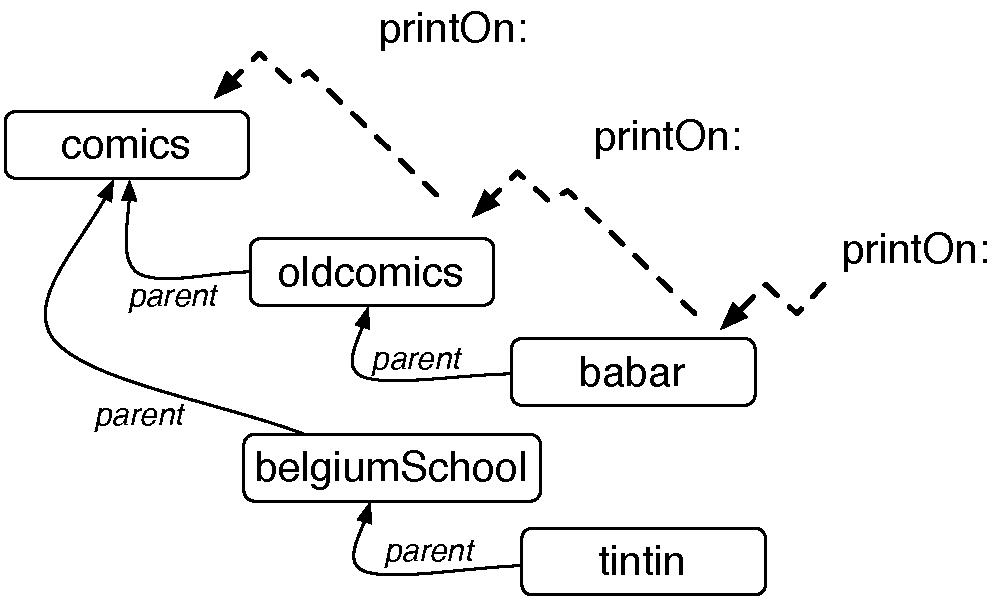
\includegraphics[width=0.6\textwidth]{/Users/ducasse/Workspace/FirstCircle/MyBooks/Bk-Writing/PharoBooks/LearningOOPWithPharoTrans/_result/pdf/Chapters/OOPNutshell/figures/InstancesRecursion2.pdf}\caption{Printing a file: Sending messages inside a graph of different objects. \label{InstancesRecursion2}}\end{center}
\end{figure}

\section{One message and multiple methods}
Before continuing let us step back and analyse the situation. We send the same messages and we execute different methods. 

\begin{displaycode}{plain}
| el1 dOldComics dComics |
el1 := MFFile new name: 'astroboy'; contents: 'The story of a boy turned into a robot that saved the world'.
dOldComics := MFDirectory new name: 'oldcomics'.
dComics := MFDirectory new name: 'comics'.
dComics addElement: dOldComics.
dOldComics addElement: el1. 
el1 printString.
>>>
'comics/oldcomics/astroboy'
\end{displaycode}

\begin{displaycode}{plain}
dOldComics printString.
>>>
'comics/oldcomics/'
\end{displaycode}

What we see is that there is one message and several implementations of methods and that sending a message will find and execute the correct method. For example, there are two methods \textcode{printOn:} one for file and one for directory but only one message \textcode{printOn:} sent from the \textcode{printString} message.

In addition a method can be defined in terms of messages sent to other objects. The method \textcode{printOn:} for directories is complex and it delegates the same message to other objects, its parents (as illustrated by Figure \ref{InstancesRecursion2}). The method \textcode{addElement:} delegates to the OrderedCollection sending a different message \textcode{add:}.
\section{Objects: stepping back}
Now that we saw some examples of objects, it is time to step back. Objects are defined by the values of their state, their behavior (shared with the other instances of their class) and an identity. 

\begin{itemize}
\item \textbf{State.} Each object has specific values. While all the instances of classes have the same structure, each instance has its own values. Each object has a private state. Clients or users of an object cannot access the state of the object if this one does not explicitly expose it by defining a method returning it (such as the message \textcode{count}).
\item \textbf{Behavior.} Each object shares the same behavior with all the instances of its class.
\item \textbf{Identity.} An object has an identity. It is unique. \textcode{oldcomics} is clearly not the same as \textcode{comics}.
\end{itemize}
\section{Examples of distribution of responsibilities }
We will now implement two functionalities: the size of directories and a search based on the contents of the files. This will set the context to explain the key concept of distribution of responsibilities.


\begin{figure}

\begin{center}
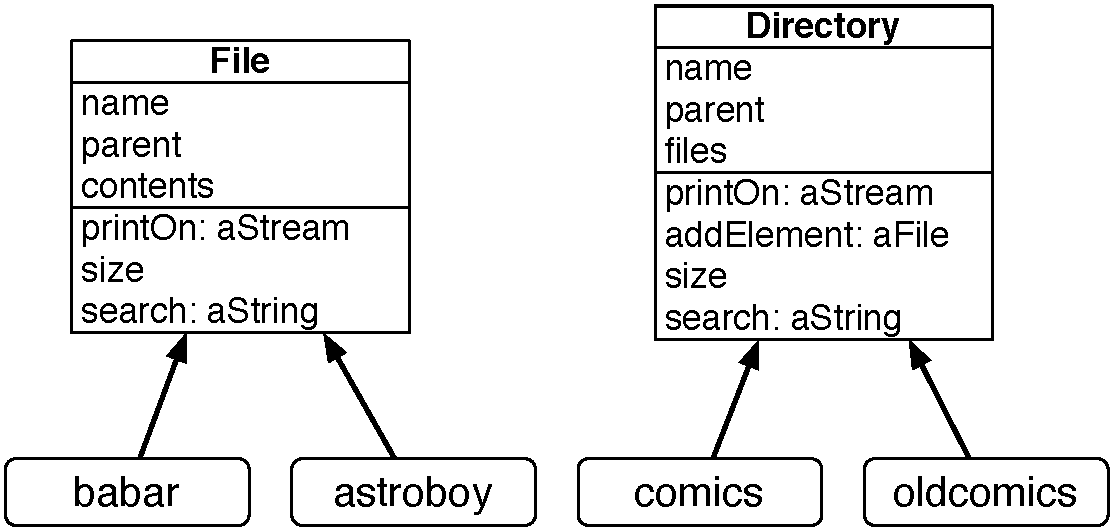
\includegraphics[width=0.6\textwidth]{/Users/ducasse/Workspace/FirstCircle/MyBooks/Bk-Writing/PharoBooks/LearningOOPWithPharoTrans/_result/pdf/Chapters/OOPNutshell/figures/FileDirectoryV1.pdf}\caption{Two classes understanding similar sets of message.\label{NutFileDirectoryV1}}\end{center}
\end{figure}

\subsection{File size }
Let us imagine that we want to compute the size of a directory. Note that the size computation we propose is fantasist but this is for the sake of the example. To perform such a computation we should also define what is the size of a file. Again let us start with examples (that you will turn into tests in the future.).

First we define the file size as the size of its name plus the size of its contents.

\begin{displaycode}{plain}
| el |
el := MFFile new name: 'babar'; contents: 'Babar et Celeste'.
el size = 'babar' size + 'Babar et Celeste' size.
>>> true
\end{displaycode}

Second we define the directory size as its name size plus the size of its files and we add and arbitrary number: 2. 

\begin{displaycode}{plain}
| p2 el |
el := MFFile new name: 'babar'.
p2 := MFDirectory new name: 'oldcomics'.
p2 addElement: el. 
p2 size = 'oldcomics' size + 'babar' size + 2
>>> true
\end{displaycode}

We define two methods \textcode{size} one for each class (see Figure \ref{NutFileDirectoryV1}).

\begin{displaycode}{plain}
MFFile >> size
	^ contents size + name size
\end{displaycode}

\begin{displaycode}{plain}
MFDirectory >> size
	| sum |
	sum := 0.
	files do: [ :each | sum := sum + each size ].
	sum := sum + name size.
	sum := sum + 2.
	^ sum
\end{displaycode}
\subsection{Search }
Let us imagine that we want to search the files matching a given string. 
Here is an example to set the stage.

\begin{displaycode}{plain}
| p el1 el2 |
p := MFDirectory new name: 'comics'.
el1 := MFFile new name: 'babar'; contents: 'Babar et Celeste'.
p addElement: el1.
el2 := MFFile new name: 'astroboy'; contents: 'super cool robot'.
p addElement: el2.
(p search: 'Ba') includes: el1
>>> true
\end{displaycode}

To implement this behavior is quite simple: we define two methods one in each class (as shown in Figure \ref{NutFileDirectoryV1}).

\begin{displaycode}{plain}
MFFile >> search: aString
	^ '*', aString, '*' match: contents
\end{displaycode}

\begin{displaycode}{plain}
MFDirectory >> search: aString
	^ files select: [ :eachFile | eachFile search: aString ]
\end{displaycode}
\section{Important points}
These two examples show several \textit{important} points:
\subsection{Modular thinking}
Each method is modular in the sense that it only focuses on the behavior of the objects specified by the class defining the method. Such method can be built by sending other messages without having to know how such methods are defined.
It also means that we can add a new kind of classes or remove one without having to change the entire system.
\subsection{Sending a message is making a choice}
We send \textit{one} message and one method amongst the \textit{multiple} methods with the same name will be selected and executed. The method is dynamically looked up during execution as we will see in Chapters \ref{cha:inheritance} and \ref{cha:messages}. Sending a message is selecting the corresponding method having the same name than the message.  When a message is sent to an object the corresponding method is looked in the class of the message receiver.

\begin{important}
Sending a message is making a choice. The system selects for us the correct method to be executed.
\end{important}
\subsection{Polymorphic objects }
We created objects (files and directories) that are \textit{polymorphic} in the sense that they offer a common set of messages (\textcode{search:}, \textcode{printOn:}, \textcode{size}, \textcode{parent:}). This is really powerful because we can compose objects (for example add a new directory or a file) without changing the program. 
Imagine that we add a new kind of directories we can introduce it and reuse extending programs based on \textcode{size} or \textcode{search:} \textit{without} changing them. 

\begin{important}
Creating polymorphic objects is a really powerful capability. It lets us extend and change programs without breaking them. 
\end{important}

Most of the time it is better to give similar name to methods performing similar behavior, and different names when the methods are doing semantically different actions, so that users of the objects are not confused. 

The  polymorphism is really a strength of object-oriented languages because it allows one to treat different objects, i.e., instances of different classes, uniformly as soon as they implement the same messages. Polymorphism works in synergy with the idea that an object is responsible to decide how to react to message reception. Indeed, the fact that different objects can implement the same messages let us write code that only tell the objects to execute some actions without worrying exactly about the kind of objects. 
\section{Distribution of responsibilities}
This example as well as the printing of files and directories illustrates something fundamental in 
object-oriented programming: the distribution of responsibilities. With the distribution of responsibilities,  each kind of objects is responsible for a specific behavior and a more elaborated behavior is composed out of such different behavior. The size of a directory is computed based on the size of its files by requesting the files to compute their size. 
\subsection{Procedural}
Let us take some time to compare with procedural thinking. Computing the size of a list of files and directories would have been expressed as a monolitic behavior sketch below:

\begin{displaycode}{plain}
sizeOfFiles: files
	| sum | 
	sum := 0.
	files do: [ :aFile | 
		aFile class = MFFile
			ifTrue: [ sum := sum + aFile name size + aFile contents size ].
		aFile class = MFDirectory
			ifTrue: [ 
				| fileSum |
				fileSum := 0.
				each files do: [:anInsideFile | fileSum := fileSum + anInsideFile name size + anInsideFile contents size ].
				sum := sum + fileSum + each name size + 2].
	^ sum	
\end{displaycode}

While this example is a bit exagerated, we see several points:

\begin{itemize}
\item First, we explicitly check the kind of structures we are manipulating. If this is a file or directory we do something different.
\item Second, the logic of the computation is defined inside the \textcode{sizeOfFiles:} itself, and not in the entities themselves.   This means in particular that such logic cannot be reused.
\item A part of the implementation logic is exposed and not in control of the object. It means that if we decide to change the internal structure of our classes, we will have to change this function too.
\item Adding a new kind of such as a root directory is not modular. We will have to modify the method \textcode{sizeOfFiles:} function.
\end{itemize}

What you should also see when you compare the two versions is that in the procedural version we have to check the kind of object we manipulate. 
In the object-oriented version, we simply tell the object to perform its own computation and return the result to us. 

\begin{important}
Don't ask, tell. Object-oriented programming essence is about sending order not checking state.
\end{important}
\section{So far so good? Not fully!}
We have a system with two classes and it offers some behavior composed out of well defined local behavior (see Figure \ref{NutFileDirectoryV1}). We can have objects composed out of other objects and messages flow within the graph. Object-oriented programming could stop here. Now it is annoying to have to duplicate structure and some methods between files and directories and this is what we will see when we will look at inheritance in Chapter \ref{cha:inheritance}.
Inheritance is a mechanism to specialize incrementally classes from other classes. 
\section{Conclusion}
\begin{itemize}
\item A class describes the state (instance variables) and the behavior (methods) of all its instances. The state of an instance is the value of its instance variables and it is specific to one single object while the behavior is shared by all the instances of a class.
\item Different objects, instances of different classes, can react differently to the same messages.
\item When sending a message, the associated method is found and executed.
\end{itemize}


% lulu requires an empty page at the end. That's why I'm using
% \backmatter here.
\backmatter

% Index would go here
\bibliographystyle{abbrv}
\bibliography{others.bib}
\end{document}
